\chapter{Modelling the 3D environment around Pulsar Wind Nebulae} \label{sec:09_multizone}

\autoref{sec:07_particle_ev} discussed how radiative and escape losses affect the energy density distribution of cosmic rays and the subsequent photon SED in a gas with constant density and magnetic field. The SED towards the extended GeV gamma-ray region to the south of \mbox{HESS\,J1825-137} was then modelled to determine the origin of cosmic rays towards this region. This is summarised in chapter \autoref{sec:08}.
\newpar
However, astrophysical environments are not uniform. For example, observatories such as Nanten (see \autoref{sec:NANTEN}) and Mopra \citep{2018PASA...35...29B} have conducted surveys of molecular and atomic gas across the Galactic plane and identified numerous structures of dense gas. Non-uniform soft photon fields such as IR and UV fields driven by star formation also provide seed photons for inverse Compton interactions, affecting the subsequent gamma-ray morphology. As discussed in \autoref{chapter_1_cr_propagation}, the magnetic field varies on a local ($<\pc$) and Galactic $>100\,\pc$ scales. In the case of PWNe, the magnetic field varies with distance to the pulsar \citep{2012SSRv..166..231R}, affecting the properties of cosmic-ray propagation out of this region (see \autoref{eq:diffusion}).
\newpar
This chapter will first discuss the transport equation that governs the time and spatial evolution of electron energy density distribution as they escape into a non-uniform environment. The chapter will then move on to describe how numerical techniques are applied to solve the transport equation. These numerical techniques are then applied to PWN \mbox{HESS\,J1825-137}, the results of which can be seen in \autoref{sec:10_second_paper}.

\section{The Transport Equation} \label{sec:09_Transport_multizone_diffusion}

\autoref{sec:chapter_7_cr_SED_evol} described the solution of the cosmic-ray energy density distribution for a simple scenario of cosmic rays being injected into a homogeneous source. However, the environment around pulsars is not uniform. The evolution of the cosmic-ray (including high-energy electrons) energy density distribution, $n$, for a non-uniform environment can be described by a Fokker-Planck equation \citep{1975MNRAS.172..557S,1978A&A....70..367C}:

\begin{equation}
    \begin{aligned}
        \pdv{n}{t}=&\pdv{ }{\gamma}\qty(\dot{\gamma}n)+\nabla\qty(\bar{\bar{D}}\cdot\nabla n)-\nabla\cdot\qty(n\vec{v}_A)-\frac{1}{3}\pdv{ }{\gamma}\qty(\gamma\qty(\nabla\cdot\vec{v}_A))n \\
        &+\pdv{ }{\gamma}\qty(\gamma^2 D_\mathrm{pp}\pdv{ }{\gamma}\qty(\frac{n}{\gamma^2})) + S\qty(\gamma,t,\vec{r})  \text{ ,}     
    \end{aligned} \label{eq:chapter_9_full_numerical_diffusion_equation}
\end{equation} 
\noindent where the first term in \autoref{eq:chapter_9_full_numerical_diffusion_equation} gives the evolution of cosmic-ray energy density distribution due to radiative losses (see chapter \autoref{sec:chapter1_non_thermal_emission}) . The second term considers the spatial evolution of cosmic rays as a second-rank tensor, $\bar{\bar{D}}\equiv\bar{\bar{D}}\qty(\gamma,t,\vec{r})$, allowing preferential direction of transport. The third term describes the evolution of the cosmic-ray density due to a co-moving fluid with velocity $\vec{v}_A$. The fourth considers losses due to adiabatic expansion. The fifth term represents the re-acceleration of cosmic rays due to stochastic processes with $D_\mathrm{pp}$ being the acceleration rate. Finally, $S\qty(\gamma,t,\vec{r})$ is the source term of high-energy cosmic rays.
\newpar
As discussed in \autoref{chapter_1_cr_propagation}, over small distances (less than the gyro-radius $r_g$), cosmic rays propagate through the ISM via ballistic motion. Over large distances, cosmic rays scatter off magnetic field turbulence and the overall propagation can be described by diffusion \citep{2015PhRvD..92h3003P}. Neglecting adiabatic losses, bulk motion and re-acceleration of cosmic rays, \autoref{eq:chapter_9_full_numerical_diffusion_equation} can be simplified to:


\begin{equation}
\begin{aligned}
\pdv{n}{t}&=\pdv{ }{\gamma}\qty(\dot{\gamma}n) + \nabla\qty(D\qty(\vec{r},\gamma)\cdot \nabla n) + S\qty(\gamma,\vec{r},t)
\end{aligned} \label{eq:chapter_9_iso_diffusion_numerical_diffusion_equation}
\end{equation} 
\noindent Note that \autoref{eq:chapter_9_iso_diffusion_numerical_diffusion_equation} is similar to \autoref{eq:chapter_7_cr_energy_distribution}, where the `escape term' has been replaced with an expression describing the losses due to diffusion. For a simple case of isotropic diffusion ($\bar{\bar{D}}\equiv D$ and $\nabla D=0$), the diffusion term in \autoref{eq:chapter_9_iso_diffusion_numerical_diffusion_equation} becomes: 

\begin{equation}
    \begin{aligned}
    \qty(\pdv{n}{t})_\text{diff}&=-\nabla\qty(D\qty(\vec{r},\gamma)\cdot \nabla n)  \\
    &=-\nabla D\cdot \nabla n -D\nabla^2 n \\
    &=-D\nabla^2 n\text{ ,} 
    \end{aligned}
\end{equation}
\noindent \autoref{eq:chapter_9_iso_diffusion_numerical_diffusion_equation} can only be solved analytically for simple scenarios (e.g. an impulsive accelerator of electrons in a medium of constant density and magnetic field, see \cite{1995PhRvD..52.3265A}). These assumptions cannot be applied to accelerators like PWNe that evolve within complex environments (see \autoref{sec:01_PWN}). Therefore, numerical methods must be applied in order to solve \autoref{eq:chapter_9_iso_diffusion_numerical_diffusion_equation}.

\subsection{Particle Transport Literature Review}

Numerical solutions of \autoref{eq:chapter_9_full_numerical_diffusion_equation} can be applied to many different scenarios in order to obtain an understanding of astrophysical phenomena. For example, \galprop is a publicly available software package that describes the propagation of cosmic rays within the Galaxy \citep{2022ApJS..262...30P}. It combines models of the cosmic-ray source distribution, interstellar gas, radiation fields and magnetic fields in order to solve the transport equation. \galprop then normalises the modelled cosmic-ray spectrum to observations at Earth in order to predict the diffuse gamma-ray emission. Other examples of software that solve the transport equation on a Galactic scale include \dragon \citep{2017JCAP...02..015E} and \picard \citep{2014APh....55...37K}. \criptic is a recent software package that simulates the propagation through complex ISM with propagation properties depending on the state of the gas \citep{2022MNRAS.517.1355K}. \criptic has been used to investigate how ISM parameters (e.g. sonic Mach number, Alfv\'en Mach number) affect the transport of cosmic rays \citep{2023MNRAS.519.1503S}.

\subsection{Numerical Solution of the Transport Equation} \label{sec:chapter_9_diffusion_numerical_sol}
\galprop, \dragon and \picard solve the transport equation on a Galactic scale ($>100\,\pc$). To understand the detailed nature and evolution of cosmic rays that escape their place of origin (e.g. PWN), the transport equation must be solved on smaller scales ($\gtrsim \pc$). To do this, finite difference techniques will be utilised to solve \autoref{eq:chapter_9_iso_diffusion_numerical_diffusion_equation}. There are other techniques used to solve differential equations (e.g. method of lines, finite volume method), however finite difference techniques are one of the most commonly used and the simplest to apply. Similarly, finite difference techniques describe a range of techniques with the simplest being the forward difference, backward difference and central difference (see \autoref{sec:A2_finite_difference}). More complex techniques, including the Euler method and Crank-Nicolson method, require the solution of linear equations, which can be computationally intensive. Therefore, a combination of the simpler techniques will be considered in this thesis. As the transport equation will be applied to the PWN \mbox{HESS\,J1825-137} in \autoref{sec:10_second_paper}, only the transport of electrons will be considered. However, these techniques also apply to the transport of cosmic-ray protons.
\newpar
Finite difference techniques obtain numerical solutions to differential equations (e.g. transport equation) by approximating derivatives with finite differences found through a Taylor series expansion (see \autoref{sec:A2_finite_difference}). To solve \autoref{eq:chapter_9_iso_diffusion_numerical_diffusion_equation} numerically, a region of interest is subdivided into a grid of voxels (a 3D pixel) of size $\Delta x \Delta y \Delta z$ as shown in \autoref{fig:chapter_8_multizone_cartesian}. The change in the electron energy distribution for a voxel at position $x$, $y$ and $z$ due to diffusion from surrounding voxels in time interval $\Delta t$ is then described by:
\begin{figure}[h!]
	\centering
	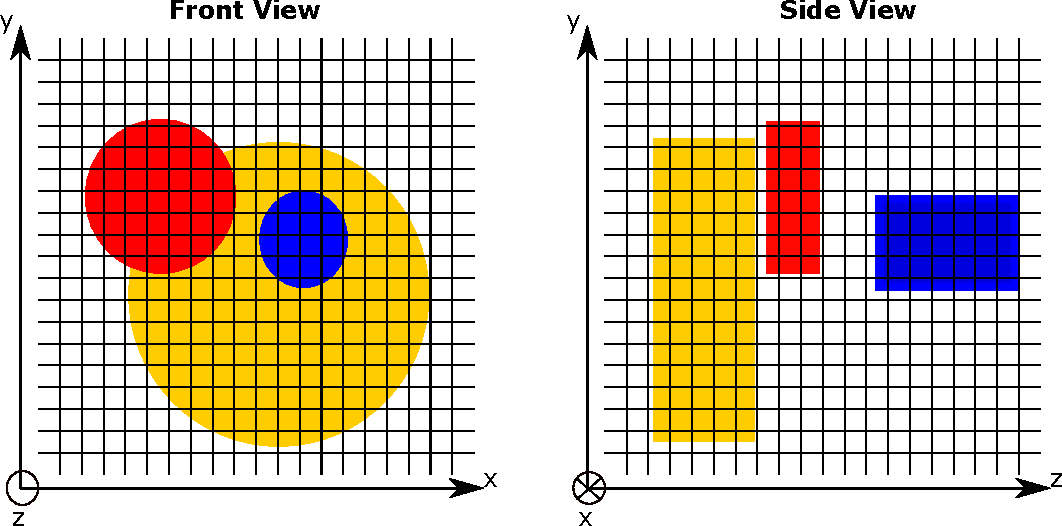
\includegraphics[width=\textwidth]{09_Multizone/Images/code/cartesian.pdf}
	\caption{Front (\textit{left}) and side (\textit{right}) view of an example region of interest showing three clouds of different densities and sizes. To numerically solve the transport equation, the region of interest is split into a 3D grid of voxels.}
	\label{fig:chapter_8_multizone_cartesian}
\end{figure}
\begin{wrapfigure}[19]{R}{0.3\textwidth}
	\centering
	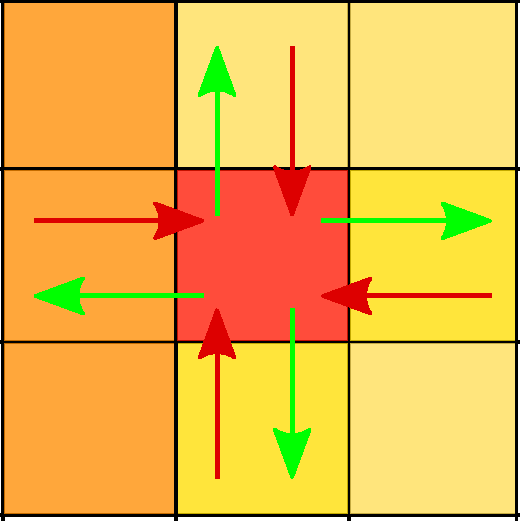
\includegraphics[width=0.29\textwidth]{09_Multizone/Images/code/transport.pdf}
	\caption{The electron energy distribution in each voxel will be calculated by tracking the flux in (red) and out (green) of neighbouring cells.}
	\label{eq:09_transport_cells}
\end{wrapfigure}
\begin{equation}
    \begin{aligned}
        \qty(\pdv{n}{t})_\text{diff}
        &= -D\nabla^2 n_\text{diff} \\
        n_\text{diff}\qty(\gamma,t+\Delta t,\vec{r})&=n_\text{diff}\qty(\gamma,t,\vec{r})+\sum_{i=x,y,z} \mathcal{D}_{i+\Delta i/2}\cdot
        \qty[n_{i+\Delta i}^{t}
        -n_{i}^t]
        +\mathcal{D}_{i-\Delta i/2}\cdot
        \qty[n_{i-\Delta i}^t
        -n_i^t]\text{ ,}
    \end{aligned} \label{eq:chapter_8_multizone_diff_numerical_sol}
\end{equation}
\noindent where
\begin{equation}
    \begin{aligned}
        \mathcal{D}_{i\pm\Delta i/2}&=\frac{D_{i\pm\Delta i}-D_i}{2} \frac{\Delta t}{\Delta i^2}\text{ ,} 
    \end{aligned} \label{eq:chapter_9_diffusion_numeric}
\end{equation}
\noindent is the dimensionless diffusion factor that considers the average magnetic field between voxel $i$ and $i\pm 1$ (see \autoref{eq:diffusion}) and $n_i^t\equiv n\qty(\gamma,r,u)$. See \autoref{eq:09_transport_cells} for a graphical description of \autoref{eq:chapter_9_diffusion_numeric}. 
\newpar 
Errors in finite difference methods arise due to the discretization of the grid and approximating partial derivatives with truncated partial derivatives (see \autoref{sec:A2_diffusion}), leading to the discrepancy between the numerical and analytical solution. Finite difference methods are said to be `stable' when the numerical solution converges to the analytical solution. Von Neumann stability analysis treats the numerical error of finite difference techniques as a time-dependent Fourier expansion and determines the condition when the error at time $t+1$ is less or equal to the error at time $t$ (see \autoref{sec:A2_finite_stability}). That is, Von Neumann stability analysis determines whether any errors due to numerical techniques are magnified in further iterations. Using Von Neumann stability analysis, \autoref{eq:chapter_8_multizone_diff_numerical_sol} is stable when:
\begin{equation}
    \begin{aligned}
    D\frac{\Delta t}{\Delta x^2}\leq \frac{1}{2}\text{ .} 
    \end{aligned} \label{eq:09_finite_difference_diff_stable}
\end{equation}
\noindent i.e. finite difference techniques can be applied to the transport equation when the diffusion coefficient, $D$, is less than or equal to half of the `maximum' diffusion coefficient (see \autoref{eq:diffusion}) implied by the voxel size and time step. Therefore, the maximum displacement of electrons across one time step is less than one voxel. If this condition is not met, electrons are transported across more than voxel. As \autoref{eq:chapter_8_multizone_diff_numerical_sol} only considers neighbouring voxels, there will be a net loss of electrons in the 3D grid.

\subsection{{\tt Multizone}} \label{sec:09_multizone_steps}

\multizone is a software originally developed by \cite{fabien} that tracks the transport and cooling of electrons in a 3D grid by applying finite difference techniques to solve \autoref{eq:chapter_8_multizone_diff_numerical_sol}. \autoref{fig:{sec:chapter_9_multizone_flow_chart}} shows the method that \multizone uses to solve \autoref{eq:chapter_8_multizone_diff_numerical_sol}.

\newcounter{counter1} %Setting counter
\newcounter{counter2} %Setting counter
\begin{enumerate}[label=\textbf{\arabic*}.]
\itemsep0em
\item The region of interest is divided into a grid of voxels of size $\Delta x\Delta y\Delta z$ of varying ISM number density and magnetic field. For simplicity, $\Delta x=\Delta y=\Delta z$. The ISM number density of each voxel can be obtained from observations of atomic and molecular gas from surveys such as Nanten (see \autoref{sec:NANTEN}). Similarly, the magnetic field of each voxel is estimated via Crutcher's relationship (see \autoref{eq:ISM_crutchers}) or assigned a value based on a specific magnetic field model (e.g. magnetic field of a PWN).
\item From \autoref{eq:diffusion}, the rate at which an electron propagates via diffusion is proportional to its energy ($D\propto E^\delta$). The 3D grid is therefore subdivided into three resolutions based on the electron energy for computational efficiency. The highest energy electrons are tracked using the grid with the lowest resolution while the slower low energy electrons are tracked on the high resolution grid. The medium and high resolution voxels have size $2\Delta x2\Delta y2\Delta z$ and $4\Delta x4\Delta y4\Delta z$ respectively (see \autoref{fig:chapter_8_multizone_resolution_cartoon}). In the context of this thesis, the high energy resolution considers electrons with energy less than $0.02\,\TeV$, the medium energy resolution considers electrons between $0.02-15\,\TeV$ and the lowest resolution considers electrons greater than $15\,\TeV$.
\item The time step used to solve \autoref{eq:chapter_8_multizone_diff_numerical_sol} is calculated (see \autoref{eq:09_finite_difference_diff_stable}) to ensure that the solution is numerically stable.
\setcounter{counter1}{\value{enumi}}
\end{enumerate}
\begin{figure}[h!]
    \centering
    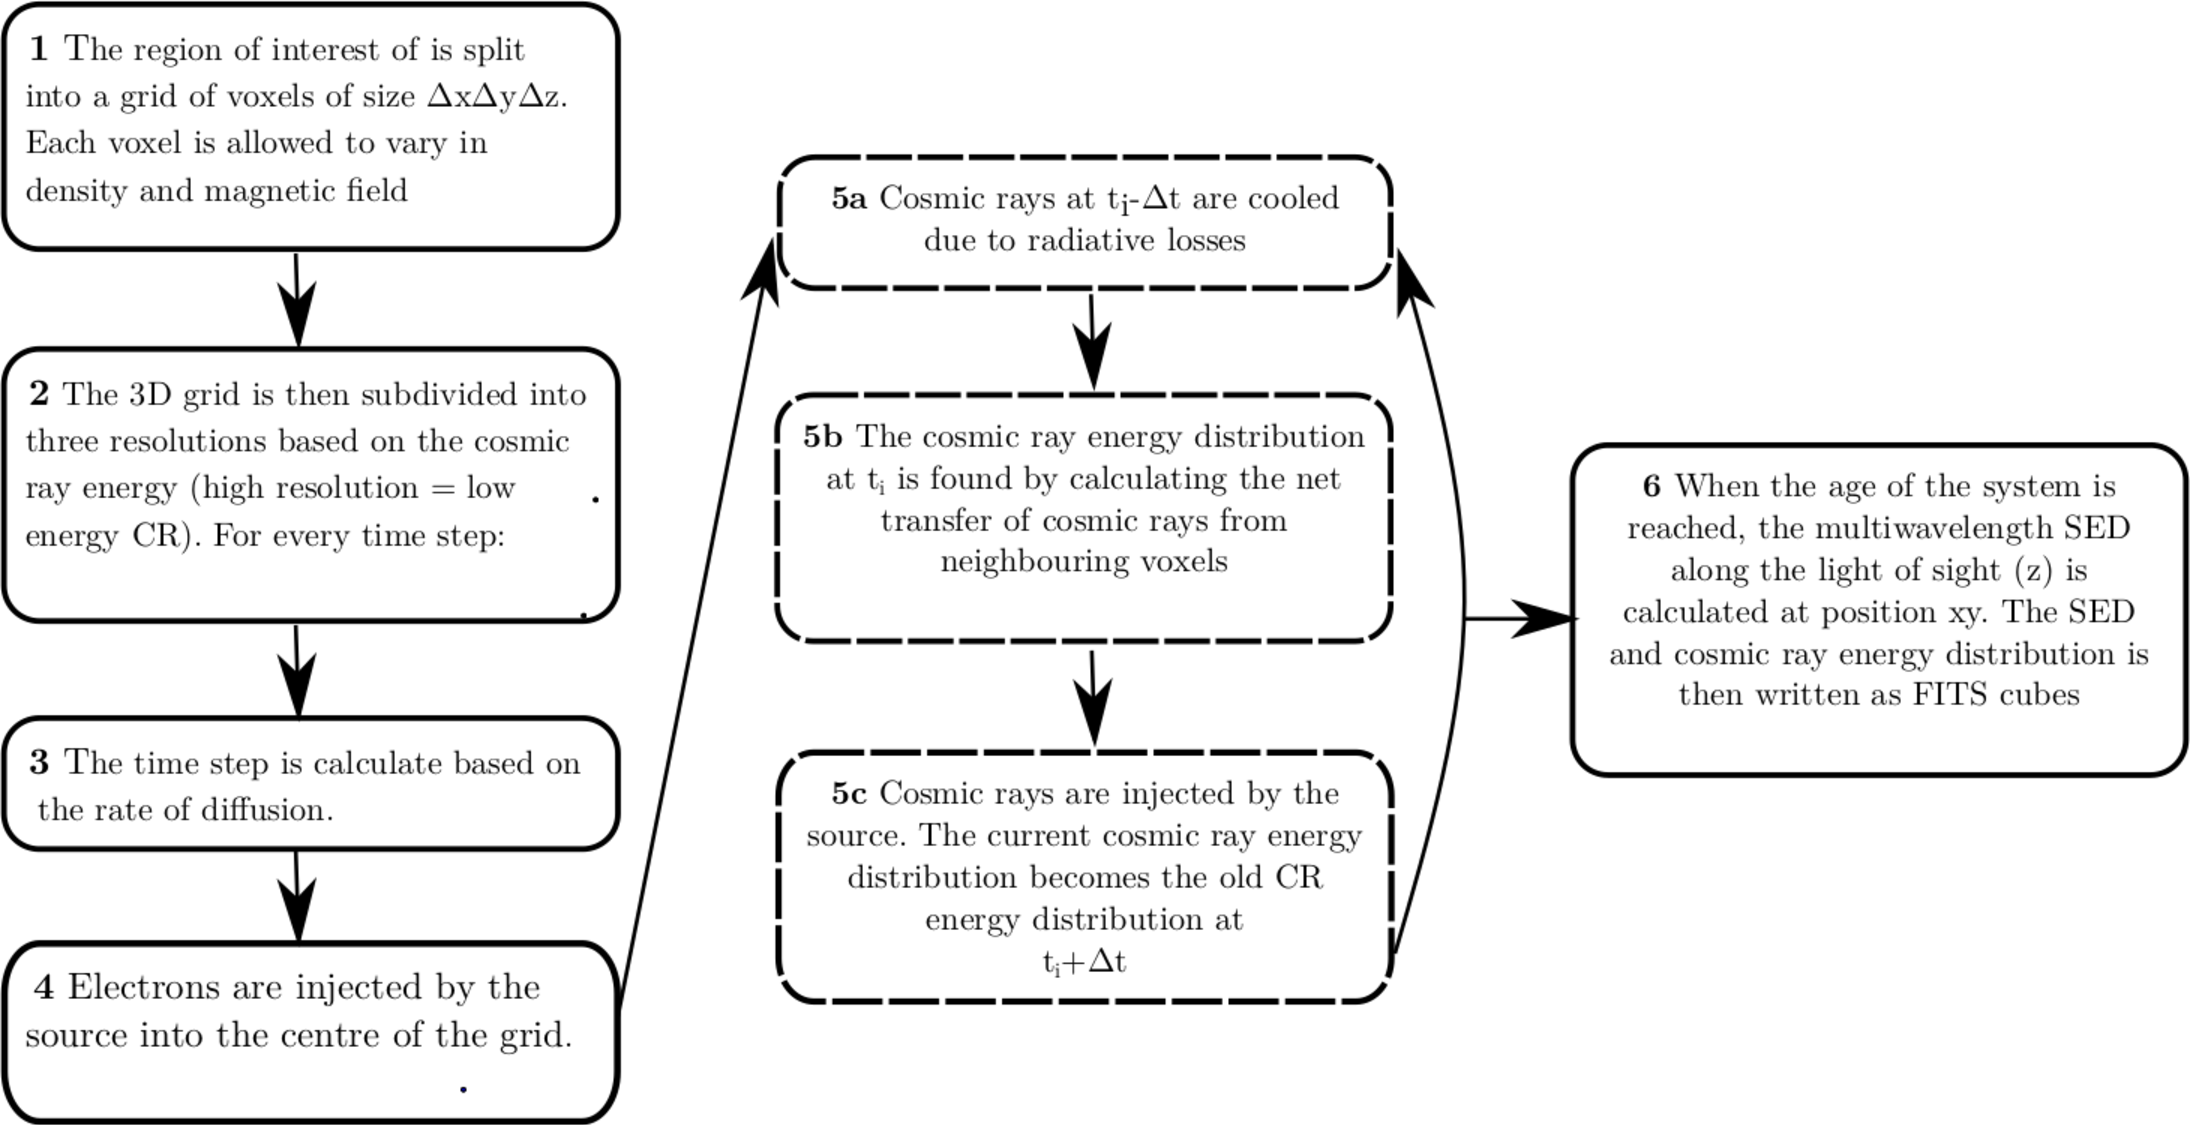
\includegraphics[width=\textwidth]{09_Multizone/Images/code/flow_chart.pdf}
    \caption{A flow-chart description of the steps {\tt Multizone} uses to calculate the electron energy distribution and subsequent SED by numerically solving the transport equation.}
    \label{fig:{sec:chapter_9_multizone_flow_chart}}
\end{figure}
\begin{figure}[h!]
    \centering
    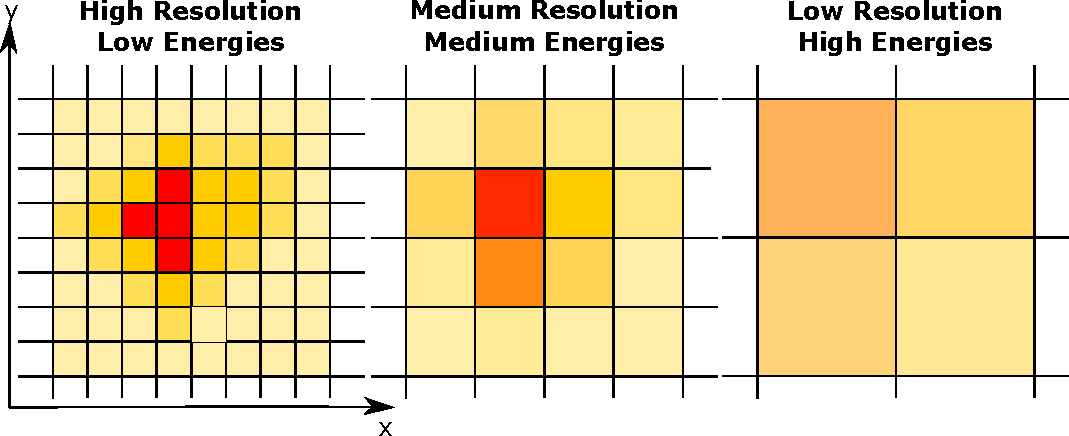
\includegraphics[width=\textwidth]{09_Multizone/Images/code/resolution_cartoon_final.pdf}
    \caption{A 2D representation of the three 3D grid resolutions used to numerically solve \autoref{eq:chapter_8_multizone_diff_numerical_sol}. Voxels with high number density or magnetic field are shown in red.}
    \label{fig:chapter_8_multizone_resolution_cartoon}
\end{figure}



\begin{enumerate}[label=\textbf{\arabic*}.]\setcounter{enumi}{\value{counter1}}
\item At $t=0$, electrons are injected into a region of size $4\Delta x4\Delta y4\Delta z$ centered on position $(x_s,y_s,z_s)$ This ensures that electrons are injected into the same region regardless of their energy. For an impulsive accelerator injecting electrons with injection luminosity $L\,\qty(\ergspersecond)$ with spectra $J'\qty(E)$ (the `de-nomalised spectra following, e.g. a power law $E^{-\Gamma}$), the total energy of electrons injected into the $4\Delta x4\Delta y4\Delta z$ cube in time interval $\Delta t$ is:
\setcounter{counter1}{\value{enumi}}
\end{enumerate}

\begin{equation}
    \begin{aligned}
        E_\text{tot}= \frac{L}{\int_{E_\text{min}}^{E_\text{max}}EJ'\qty(E)\dd{E}} \Delta t\text{ ,} 
    \end{aligned} \label{eq:09_multizone_total_energy_in_cells}
\end{equation}

\begin{enumerate}[label=\textbf{\arabic*}.]\setcounter{enumi}{\value{counter1}}
\item[] where $E_\text{min}$ and $E_\text{max}$ are the minimum and maximum electron energy injected into the grid respectively.
\item For every time step:
\setcounter{counter1}{\value{enumi}}
\end{enumerate}
\begin{enumerate}[label=\textbf{\arabic*}]\setcounter{enumi}{\value{counter1}}
	\item[]
\begin{enumerate}[label*=\textbf{\alph*}.]
    \itemsep0em
    \item The energy loss of electrons from the previous time step is calculated. As {\tt Multizone} treats continuous injectors as a series of impulsive injections, the electron energy distribution due to radiative losses during time $\Delta t$ is: \label{item:09_step_5a}
    \setcounter{counter2}{\value{enumii}}
\end{enumerate}
\end{enumerate}

\begin{equation}
    \begin{aligned}
    n\qty(\gamma,t+\Delta t) &=\frac{\dot{\gamma}_t}{\dot{\gamma}_{t+\Delta t}}n\qty(\gamma,t,\vec{r})\text{ ,} 
    \end{aligned}
\end{equation}

\begin{enumerate}[label=\textbf{\arabic*}]
\itemsep0em
\setcounter{enumi}{\value{counter1}}
\item[]
\begin{enumerate}[label*=\textbf{\alph*}.]\setcounter{enumii}{\value{counter2}}
    \itemsep0em
    \item[] where $\gamma_t$ is the Lorentz factor of the electron at time $t$ before cooling to Lorentz factor $\gamma_{t+\Delta t}$  (see \autoref{eq:chapter_7_cooling_time}). 
    \item For each voxel, the electron energy distribution at time $t + \Delta t$ is found by incrementing the electron energy distribution from step \ref{item:09_step_5a} with the net transfer of electrons from neighbouring voxels with (see \autoref{eq:chapter_8_multizone_diff_numerical_sol}).
    \item Electrons are injected into the grid with total energy given by \autoref{eq:09_multizone_total_energy_in_cells}. The current electron energy distribution becomes the `old' electron energy distribution for the next time step.
\end{enumerate}
\setcounter{counter1}{\value{enumi}}
\end{enumerate}
\begin{enumerate}[label=\textbf{\arabic*}.]\setcounter{enumi}{\value{counter1}}
\item When the desired age is reached (e.g. the estimated age of \mbox{HESS\,J1825-137} is $21-40\,\kiloyear$), the subsequent photon SED emitted by each voxel is calculated and summed along the line of sight. The photon SED and electron energy distribution are then written as FITS cubes for further analysis.
\end{enumerate}

\subsection{Analytical Solution: Diffusion-only} \label{sec:09_multizone_diffusion_only}

The numerical solution ({\tt Multizone}) will now be compared to a diffusion-only scenario (no radiative losses) for an impulsive accelerator injecting electrons at $x=y=z=t=0$. The analytical solution of \autoref{eq:chapter_9_iso_diffusion_numerical_diffusion_equation} for a diffusion-only scenario (\autoref{eq:chapter_7_R_ev_green_solution} when $t\ll \gamma/\dot{\gamma}=\tau$) is:

\begin{equation}
    \begin{aligned}
        n\qty(E,t,r)&=n_0\qty(\frac{1}{4\pi Dt})^\frac{3}{2}\exp(-\frac{r^2}{4Dt})\text{ ,} 
    \end{aligned} \label{eq:09_multizone_diff_only_sol}
\end{equation}
\noindent where $r^2=x^2+y^2+z^2$.

\begin{figure}[h!]
    \centering
    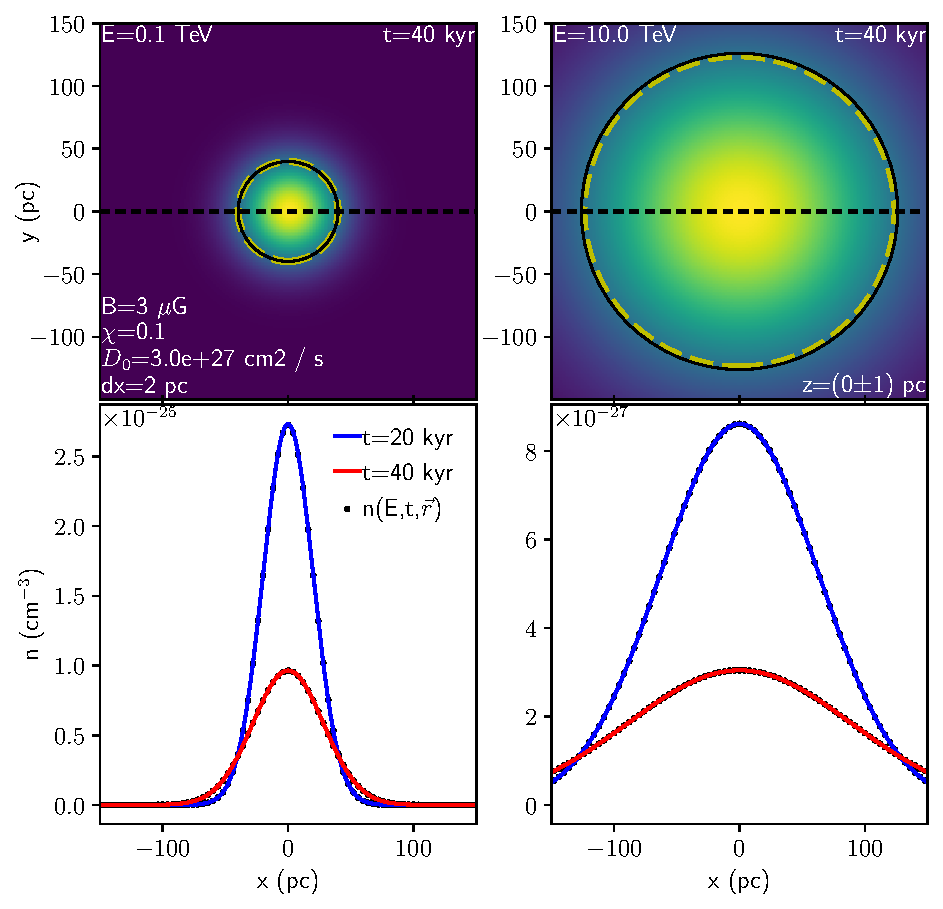
\includegraphics[width=\textwidth]{09_Multizone/Images/diffusion/diffusion_3D_multizone_final.pdf}
    \caption{Distribution of electrons injected into a 3D grid at $x=y=z=t=0$ and subjected to diffusion. (\textit{Top}) The number density distribution taken at slice $z=(0\pm 1)\,\pc$ and time $40\,\kiloyear$. The black and yellow dashed circles represent the 2D variance radius ($R_\text{var}$) and the radius containing $1\sigma=68\%$ of electrons ($R_\sigma$) in the 2D slice respectively. (\textit{Bottom}) Comparing the numerical solution (lines) and analytical solution (dots, see \autoref{eq:09_multizone_diff_only_sol}) at $t=20$ and $40\,\kiloyear$ along $y=(0\pm 1)\,\pc$ (dashed horizontal line in the bottom panel).}
    \label{fig:09_multizone_diff_3D}
\end{figure}
\newpar 
\autoref{fig:09_multizone_diff_3D} compares the numerical and analytical solution for model parameters applicable to the region towards \mbox{HESS\,1825-137} (see \autoref{sec:10_second_paper}). Electrons are injected into a uniform ISM with a magnetic field taking the Galactic average of $3\,\si{\micro G}$ \citep{2002cra..book.....S} and diffusion suppression factor $\chi=0.1$. A time step of $8\,\si{yr}$ and voxel width of $\Delta x=\Delta y=\Delta z = 2\,\pc$ was chosen such that the finite difference method is stable for electrons $\lesssim 600\,\TeV$ (see \autoref{eq:09_finite_difference_diff_stable}). The bottom panels of \autoref{fig:09_multizone_diff_3D} show the number density distribution taken at slice $z=\qty(0\pm 1)\pc$ for electron energies $0.1$ and $10\,\TeV$ and age $t=40\,\kiloyear$. Note that the radius containing $1\sigma=68\%$ of electrons ($R_\sigma$) in the 2D slice is equivalent to the 2D variance radiance ($R_\text{var}=\sqrt{4Dt}$) for both energies. Similarly, the top panels show that the numerical solution is able to closely match the analytical solution for a slice taken at $y=z=(0\pm 1)\,\pc$.
\newpar 
The variance of the $68\%$ containment radius of \autoref{eq:09_multizone_diff_only_sol} is given by (see \autoref{sec:A5_variance}):

\begin{equation}
	\begin{aligned}
		\mathrm{Var}\qty(r)&=6Dt\text{ .} 
	\end{aligned}
\end{equation}
\noindent i.e. $68\%$ of electrons are contained within 3D radius of $R_\text{var}=\sqrt{6Dt}$. The 2D variance radius for a slice in the 3D grid (e.g. $z=(0\pm 1)\,\pc$) is given by:
\begin{equation}
	\begin{aligned}
		\mathrm{Var}\qty(r)&=\sqrt{4Dt}\text{ .} 
	\end{aligned}
\end{equation}


\subsection{Diffusion and Radiative Energy Losses: Analytical and Numerical Solution Comparison}

Next, finite difference techniques will be used to predict the electron number density for a diffusive scenario including radiative energy losses for a constant ISM and magnetic field (see \autoref{sec:chapter_1_leptonic_gre}).
\newpar
An impulsive accelerator will inject electrons with spectra $=AE^{-\Gamma}$ into a volume of size $4\,\pc \times 4\,\pc \times 4\,\pc$ at $t=0$. The analytical solution can be found by convolving the Green's solution of the transport equation (see \autoref{eq:chapter_7_crpropev_leptonic_impulsive}) with the radius of the electron injector $R_\text{source}$:

\begin{equation}
	\begin{aligned}
		n\qty(\gamma,t,x,y,z)&=\iiint_{x,y,z=-\infty}^{\infty} n_\text{green}\qty(\vec{r}-\vec{s}_r)R_\text{source}\qty(\vec{s}_r)\dd{\vec{s}_r} \text{ ,} 
	\end{aligned} \label{eq:chapter_9_multizone_diff_exact}
\end{equation}
\noindent where:

\begin{equation}
    \begin{aligned}
    R_\text{source}\qty(\vec{s}_r)=
    \begin{cases}
    1\text{, }-2\,\pc\leq s_r\leq 2\,\pc \\
    0\text{, }\quad\text{otherwise}
    \end{cases}\text{ ,} 
    \end{aligned} \label{eq:09_multizone_source_func}
\end{equation}
\noindent and

\begin{equation}
    \begin{aligned}
        n_\text{green}\qty(\gamma,t,r)&=\frac{\qty(1-\gamma b_st)^{\Gamma-2}A\gamma^{-\Gamma}}{\pi^{\frac{3}{2}}R_\text{diff}\qty(\gamma,t,B)^3}\exp\qty(-\frac{r^2}{R_\text{diff}\qty(\gamma,t,B)^2}) \\
        &=\frac{n_0}{\pi^{\frac{3}{2}}R_\text{diff}\qty(\gamma,t,B)^3}\exp\qty(-\frac{r^2}{R_\text{diff}\qty(\gamma,t,B)^2}) \\
        R_\text{diff}&=\sqrt{\frac{4D\qty(\gamma,B)}{b_s\gamma\qty(1-\delta)}\qty[1-\qty(1-\gamma b_s t)^{1-\delta}]}\text{ ,} 
    \end{aligned} \label{eq:09_multizone_green_rad_loss}
\end{equation}
\noindent where $A$, $b_s$, ect. are defined in \autoref{sec:chapter_7_cr_SED_evol}. As with \autoref{sec:09_multizone_diffusion_only}, electrons will be injected into a uniform ISM (i.e constant density $n_0$ and magnetic field $B$). Combining \autoref{eq:chapter_9_multizone_diff_exact}, \autoref{eq:09_multizone_source_func} and \autoref{eq:09_multizone_green_rad_loss}:

\begin{equation}
	\begin{aligned}
		n_\text{exact}\qty(\gamma,t,x,y,z)&=\int_{x=-2}^{2}\int_{y=-2}^{2}\int_{z=-2}^{2}\frac{n_0}{64\pi^{\frac{3}{2}}R_\text{diff}^3}\prod_{i=x,y,z} \exp(-\frac{\qty(i-s_i)^2}{R_\text{diff}^2})\dd{s_i}\text{ ,} 
	\end{aligned} \label{eq:chapter_9_multizone_diff_exact2}
\end{equation}
\noindent where $i=x,y,z$. Using a change of variables:

\begin{equation}
	\begin{aligned}
		u_i&=\frac{i-s_i}{R_\text{diff}} \\
		\therefore \dd{s_i}&=-R_\text{diff}\dd{u_i}\text{ .} 
	\end{aligned}
\end{equation}
\noindent \autoref{eq:chapter_9_multizone_diff_exact2} becomes:

\begin{equation}
	\begin{aligned}
		n_\text{exact}\qty(\gamma,t,x,y,z)&=\frac{n_0}{64\pi^{\frac{3}{2}}}\prod_{i=x,y,z}\int_{\frac{i-2}{R_\text{diff}}}^{\frac{i+2}{R_\text{diff}}}\exp(-u_i^2)\dd{u_i}\text{ .} 
	\end{aligned} \label{eq:09_diff_losses_temp}
\end{equation}
\noindent From the definition of the error function:

\begin{equation}
    \begin{aligned}
    \erf(a)&= \frac{2}{\sqrt{\pi}}\int_{0}^{a}\exp(-t^2)\dd{t}\text{ .} 
    \end{aligned}
\end{equation}
\noindent The analytical solution can be simplified to:

\begin{equation}
	\begin{aligned}
		n_\text{exact}\qty(\gamma,t,x,y,z)&=\frac{n_0}{64\pi^{\frac{3}{2}}}\prod_{i=x,y,z}\int_{\frac{i-2}{R_\text{diff}}}^0\exp(-u_i^2) + \int_{0}^{\frac{i+2}{R_\text{diff}}}\exp(-u_i^2) \\
		&=\frac{n_0}{512} \prod_{i=x,y,z} \erf\qty(\frac{i+2}{R_\text{diff}})-\erf\qty(\frac{i-2}{R_\text{diff}})\text{ .} 
	\end{aligned} \label{eq:chapter_9_multizone_diff_exact_sol}
\end{equation} 

\autoref{fig:09_multizone_diff_exact_convergence} shows the time it takes for the the numerical solution of the electron energy distribution to `converge' to the analytical solution (\autoref{eq:chapter_9_multizone_diff_exact_sol}) for a situation with the same parameters as \autoref{fig:09_multizone_diff_3D} but including energy losses due to synchrotron radiation. It can be noted that the numerical solution tends to under-predict the analytical solution before converging, where the convergence time is proportional to the distance from the
\begin{figure}[h!]
	\centering
	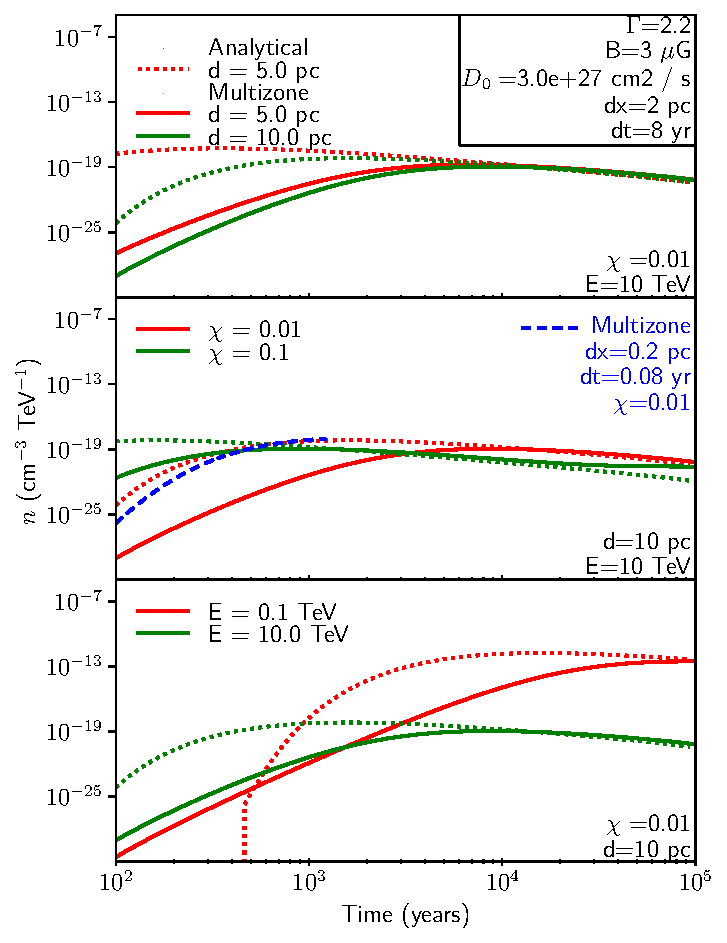
\includegraphics[width=0.7\textwidth]{09_Multizone/Images/diffusion/analytical_diff_convergence.pdf}
	\caption{Evolution of the impulsive electron energy density distribution for the analytical solution (filled dots) and numerical solution (solid lines) with the same parameters to \autoref{fig:09_multizone_diff_3D}. The top panel shows the evolution at distance $5\,\pc$ and $10\,\pc$ from the source. The middle panel compares the evolution for a situation where $\chi=0.01$ and $\chi=0.1$. The blue dashed line represents the numerical solution for $\chi=0.01$ with a time and spatial resolution of $\dd{t}=0.08\,\si{yr}$ and $\dd{x}=0.2\,\pc$ respectively. The bottom panel compares the evolution for electrons with energy $E=0.1\,\TeV$ and $10\,\TeV$.}
	\label{fig:09_multizone_diff_exact_convergence}
\end{figure} 
source (top-panel), diffusion suppression factor (middle-panel) and inversely proportional to the energy (bottom panel). The blue dashed line in the middle panel shows the numerical solution for $\chi=0.01~$ with a finer time and spatial resolution. The convergence time for the fine ($\dd{x}=0.2\,\pc$, $\dd{t}=0.08\,\si{yr}$) and coarse ($\dd{x}=2\,\pc$, $\dd{t}=8\,\si{yr}$) resolution are $\approx 0.4\,\si{kyr}$ and $\approx 12.8\,\si{kyr}$ respectively. Note that the numerical solution starts to diverge after $30\,\kiloyear$ for $\chi=0.1$ and electron energy of $10\,\TeV$ (middle-panel). Divergence occurs when the variance radius $R_\text{var}=\sqrt{6Dt}$ is approximately half the width of the grid, i.e. the time it takes electrons to reach the simulated boundary. For the aforementioned example, this occurs at approximately $10\,\kiloyear$. Therefore, the numerical solution must employ a grid size larger than the diffusion variance radius.
\begin{figure}[h!]
    \centering
    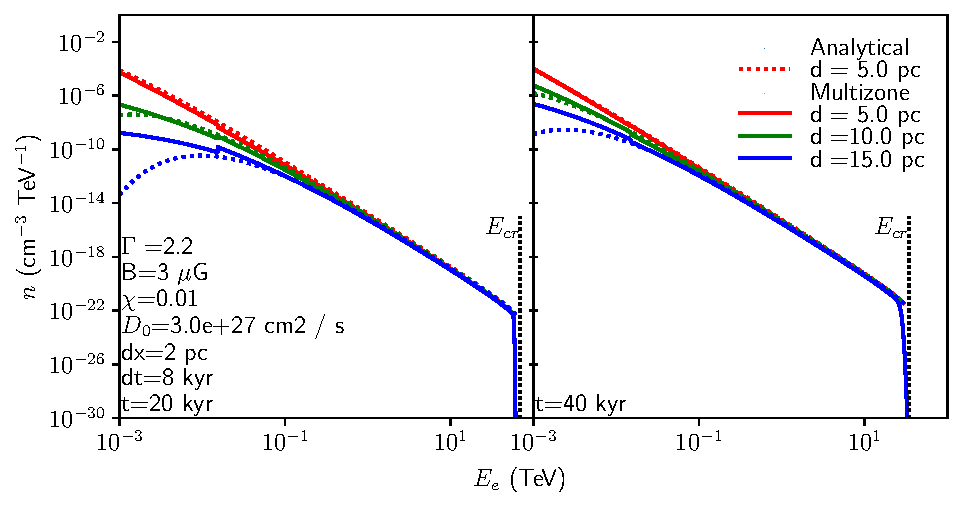
\includegraphics[width=1.0\textwidth]{09_Multizone/Images/diffusion/analytical_diff_sol.pdf}
    \caption{Energy distribution of electrons $20\,\kiloyear$ (\textit{left}) and $40\,\kiloyear$ (\textit{right}) after an impulsive accelerator injects electrons into a system with the same parameters as \autoref{fig:09_multizone_diff_3D}. The electron energy distribution of electrons is taken  $5\,\pc$ (red), $10\,\pc$ (green) and $15\,\pc$ (blue) from the accelerator with the analytical and numerical solutions being represented by the circles and solid lines respectively. The vertical black dotted lines represents the critical energy $E_\text{cr}$ of electrons (see \autoref{eq:chapter_7_imp_lep_critical_lorentz}).}
    \label{fig:09_multizone_diff_exact_energy}
\end{figure}
\newpar 
\autoref{fig:09_multizone_diff_exact_energy} compares the analytical solution of the electron energy distribution (\autoref{eq:chapter_9_multizone_diff_exact_sol}) and the energy distribution predicted by the numerical solution for ages $20\,\kiloyear$ and $40\,\kiloyear$ with the same parameters as per \autoref{fig:09_multizone_diff_3D}. The numerical solution is able to match the critical energies (the maximum energy of electron due to energy losses, see \autoref{eq:chapter_7_imp_lep_critical_lorentz}) of $\approx 70\,\TeV$ and $\approx 35\,\TeV$ after $20\,\kiloyear$ and $40\,\kiloyear$ respectively. The $20\,\kiloyear$ and $40\,\kiloyear$ numerical solution at a distance of $5\,\pc$ from the accelerator follows the analytical solution. However, the numerical solution under-predicts the electron energy distribution for energies $\lesssim 0.1\,\TeV$ at a distance of $10\,\pc$ and $15\,\pc$. In these cases, the $d=10\,\pc$ and $d=15\,\pc$ numerical solutions for electrons with energies $\lesssim 0.1\,\TeV$ have not yet `converged' to the analytical solution. However, these electrons will interact with the CMB via IC interactions to produce photons with energies less than $100\,\MeV$ (see \autoref{eq:01_non_thermal_IC_max}) which lies at the lower end of \textit{Fermi}-LAT's sensitivity and flux points extracted from \mbox{HESS\,J1825-137} (see \autoref{fig:chapter1_hess_j1825_morphology_paramaters}). A finer grid resolution and time step would be needed for the numerical solution to predict the analytical solution at these energies as seen in \autoref{fig:09_multizone_diff_exact_convergence}. However, this is left to future work as the focus of this thesis is on $\TeV$ electron energies.

%%%%%%%%%%%%%%%%%%%%%%%%%%%%%%%%%%%%%%%%%%%%%%%%%%%%%%%%%%%%%%%%%%%%%%%%%%%%%%%%%%%%%%%%%%%%%%%%%%%%%%%%%%%
\section{Advection} \label{sec:09_advection}

\begin{SCfigure}[0.5][b!]
    \centering
    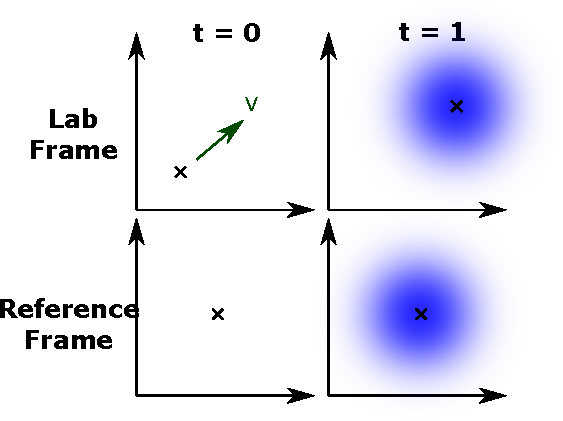
\includegraphics{09_Multizone/Images/advection/adv_example.pdf}
    \caption{Advection of electrons in the lab frame due to impulsive injector (cross) moving at velocity $v$ in lab frame.}
    \label{fig:09_multizone_adv_edxample}
\end{SCfigure}

\autoref{sec:09_Transport_multizone_diffusion} only considered a simple case of isotropic diffusion, where the diffusion tensor in \autoref{eq:chapter_9_full_numerical_diffusion_equation} becomes a scalar ($\bar{\bar{D}}\equiv D$). In this case, the overall net motion of the electron population is zero, i.e. the average position of the electrons does not change (see \autoref{fig:09_multizone_diff_3D}). However, this is not always the case. Consider an impulsive injector of cosmic rays moving at velocity $v$ in the laboratory frame (see the example in \autoref{fig:09_multizone_adv_edxample}). The average position of cosmic rays remains constant in the reference frame of the injector. While in laboratory frame, the average position of cosmic rays changes with time where the overall bulk particle flow is defined as advection.
\newpar
Anisotropic diffusion describes a situation where cosmic rays have a preferential direction of diffusion. This can be due to the presence of strong magnetic field lines, inhibiting transport perpendicular to the magnetic field (see \cite{2013ApJ...768...73M,2013MNRAS.429.1643N,2023arXiv230402684L}) or some asymmetric force as typically seen in PWN. If diffusion is anisotropic then the second term in \autoref{eq:chapter_9_full_numerical_diffusion_equation} becomes:

\begin{equation}
    \begin{aligned}
        \qty(\pdv{n}{t})_\text{diff}&=\nabla\qty(\bar{\bar{D}}\cdot\nabla n)
        &=\nabla\bar{\bar{D}}\cdot\nabla n+\bar{\bar{D}}\cdot\nabla^2 n\text{ .} 
    \end{aligned} \label{eq:09_anisotropic_diffusion}
\end{equation}
 \noindent Note that \autoref{eq:09_anisotropic_diffusion} is similar to the transport equation that considers both advection and isotropic diffusion:

 \begin{equation}
     \begin{aligned}
         \qty(\pdv{n}{t})_\text{diff+adv}&=\nabla\cdot\qty(n\vec{\nu}_A)+D\nabla^2 n\text{ .} 
     \end{aligned}
 \end{equation}
\noindent i.e. anisotropic diffusion can be approximated by isotropic diffusion with an advective component (as in the case of \autoref{fig:09_multizone_adv_edxample}).
\newpar 
Several astrophysical environments show a preferential direction of particle transport. For example, the geometry of SNRs and the surrounding medium can affect the transport of protons out of the system and the subsequent shape of the SNR (e.g. \cite{2015MNRAS.450.3080M,2021ApJ...923..233G}). Such SNRs include the young \mbox{SNR\,G1.9+0.3}, \mbox{SNR\,G296.5+10.0} and the Cygnus loop nebula. Advection may be of particular importance to PWNe. For example the asymmetric gamma-ray morphology towards PWN \mbox{HESS\,J1825-137} \citep{2019A&A...621A.116H} implies a bulk motion of particles towards lower Galactic longitudes with total velocity ($v=v_\text{adv}+v_\text{diff}$) of $0.01c$ \citep{2019A&A...621A.116H}. In general, it has been proposed that advection dominates the particle transport close to the pulsar, while diffusion dominates the outer reaches of the nebula \citep{2020A&A...636A.113G,2021PhRvD.104l3017R}. This section will describe the finite difference techniques used to solve \autoref{eq:chapter_9_full_numerical_diffusion_equation} that includes a bulk advective transport of electrons.

\subsection{Numerical Solution} \label{sec:09_multizone_advection_num_sol}

The advective component of \autoref{eq:chapter_9_full_numerical_diffusion_equation} is:

\begin{equation}
    \begin{aligned}
    \qty(\pdv{n}{t})_\text{adv}&=-\nabla\cdot\qty(n\vec{v}_A)\text{ ,} 
    \end{aligned} \label{eq:09_multizone_adv}
\end{equation}
\noindent where $\vec{v}_A\equiv [v_\text{A,x},v_\text{A,y},v_\text{A,z}]$ is the velocity of the bulk flow. Taking the simple case where $v_A$ is constant over time and both energetically and spatially independent, \autoref{eq:09_multizone_adv} becomes:

\begin{equation}
    \begin{aligned}
    \qty(\pdv{n}{t})_\text{adv}&=-\vec{v}_A\nabla n\text{ .} 
    \end{aligned} \label{eq:chapter_9_advection_component}
\end{equation}
\noindent For a scenario considering advection and isotropic diffusion, diffusion is the dominant particle transport process for higher energy particles (when $R_\text{diff}>v_At$) and advection dominating at lower energies ($R_\text{diff}<v_At$). For the 3D grid described in \autoref{sec:chapter_9_diffusion_numerical_sol}, the advective change in the electron energy distribution due to the surrounding voxels in time $\Delta t$ is described by (see \autoref{sec:A2_advection}):

\begin{equation}
    \begin{aligned}
        n_\text{adv}\qty(\gamma,t+\Delta t,\vec{r})&=n_\text{adv}\qty(\gamma,t,\vec{r})+\sum_\qty{i=x,y,z}v_{A,i}\frac{\Delta t}{\Delta i}
        \begin{cases}
            \qty(n_{i+\Delta i}^t-n_{i}^t)\text{,}& v_\text{A,i}<0 \\
            \qty(n_{i}^t-n_{i-\Delta i}^t)\text{,}& v_\text{A,i}>0
        \end{cases} \text{ ,}
    \end{aligned} \label{eq:chapter_9_multizone_adv_numerical_sol}
\end{equation}
\noindent where the forward difference method (i.e. using cells $i$ and $i+\Delta i$ to approximate the derivative) is used when $v_\text{A,i}<0$ and the backward difference method (i.e. using cells $i$ and $i-\Delta i$) is used when $v_\text{A,i}>0$. 
\newpar 
Using Von Neumann stability analysis (see \autoref{eq:A3_advection_stability}), \autoref{eq:chapter_9_multizone_adv_numerical_sol} is stable when:

\begin{equation}
    \begin{aligned}
    \Delta t \leq \frac{\Delta i}{\abs{v_{A,i}}}\text{ .} 
    \end{aligned} \label{eq:09_multizone_advection_stability}
\end{equation}
\noindent i.e. the distance travelled by a cosmic ray in one time step must be less than the size of one voxel.

\subsection{Analytical Solution} \label{sec:09_multizone_adv}

Consider 1D advection, the analytical solution to \autoref{eq:09_multizone_adv} is simply:

\begin{equation}
    \begin{aligned}
        n\qty(t,x)&=n\qty(t=0,x-vt)\text{ .} 
    \end{aligned}
\end{equation}

\noindent i.e. by assuming $v_A$ is constant, advection is simply a translation in space. However, the discetization of space can lead to dispersion in the numerical solution. If $\Delta t = \Delta x/v$, electrons are translated exactly one voxel for each time step as shown in the upper panels of \autoref{fig:09_multizone_smearing}. But when $\Delta t < \Delta x/v$, electrons are transported less than the voxel width and the numerical solution effectively begins to `disperse' particles as shown in the lower panels of \autoref{fig:09_multizone_smearing}.
\begin{figure}[h!]
    \centering
    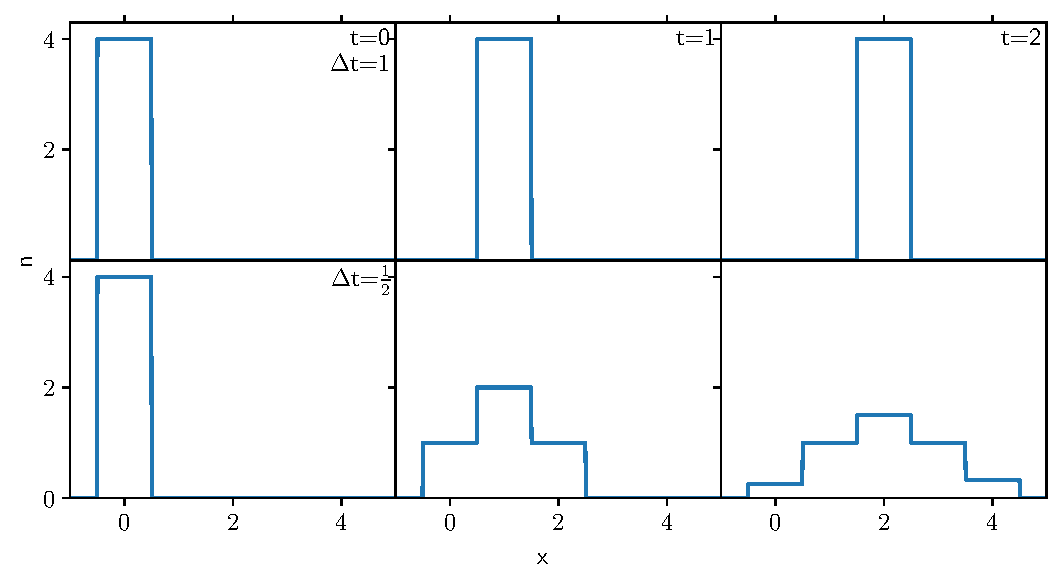
\includegraphics[width=\textwidth]{09_Multizone/Images/advection/advection_smearing.pdf}
    \caption{The application of finite difference methods for an initial distribution following distribution ($n(-0.5<=x<0.5)=4$) at $t=0$ with velocity $v=1$. The voxel width ($\Delta x=1$) remains constant while the time steps are $1$ (\textit{top}) and $0.5$ (\textit{bottom}).}
    \label{fig:09_multizone_smearing}
\end{figure}
\newpar 
To understand the origins of the dispersion, consider \autoref{eq:chapter_9_advection_component} where the time derivative is replaced by the forward difference (see \autoref{eq:A2_forward_tecnique}) and the space derivative has been replaced by the backwards derivative (i.e. when $v>0$):

\begin{equation}
    \begin{aligned}
        \frac{n_i^{t+\Delta t}-n_{i}^{t}}{\Delta t}&=-\frac{v}{\Delta i} \qty(n_{i}^t-n_{i-\Delta i}^t)\\
        \frac{1}{2\Delta t} \qty(n_{i}^{t+\Delta t}+n_{i}^{t+\Delta t}-n_{i}^{t-\Delta t}+n_{i}^{t-\Delta t}-2n_{i}^{t}) &=-\frac{v}{2\Delta i} \qty(2n_{i}^t-n_{i-\Delta i}^t-n_{i-\Delta i}^t-n_{i+\Delta i}^t+n_{i+\Delta i}^t) \\
        \frac{1}{2\Delta t}\qty(\qty[n_{i}^{t+\Delta t}-n_{i}^{t-\Delta t}]+\qty[n_{i}^{t+\Delta t}+n_{i}^{t-\Delta t}-2n_{i}^{t}])&=-\frac{v}{2\Delta i} \qty(\qty[n_{i+\Delta i}^t-n_{i-\Delta i}^t]-\qty[n_{i+\Delta i}^t+n_{i-\Delta i}^t-2n_{i}^t]) \text{ .} 
    \end{aligned} \label{eq:09_multizone_dispersion_ex}
\end{equation}

Similarly, if the spatial derivative \autoref{eq:09_multizone_dispersion_ex} is approximated by the backward difference (when $v<0$):

\begin{equation}
    \begin{aligned}
        \frac{n_i^{t+\Delta t}-n_{i}^{t}}{\Delta t}&=-\frac{v}{\Delta i} \qty(n_{i+\Delta i}^t-n_{i}^t)\\
        \frac{1}{2\Delta t}\qty(\qty[n_{i}^{t+\Delta t}-n_{i}^{t-\Delta t}]+\qty[n_{i}^{t+\Delta t}+n_{i}^{t-\Delta t}-2n_{i}^{t}])&=-\frac{v}{2\Delta i} \qty(\qty[n_{i+\Delta i}^t-n_{i-\Delta i}^t]+\qty[n_{i+\Delta i}^t+n_{i-\Delta i}^t-2n_{i}^t]) \text{ .} 
    \end{aligned} \label{eq:09_multizone_dispersion_ex2}
\end{equation}

In the continuous limit:

\begin{subequations}
    \begin{alignat}{1}
        n_{i}^{t+\Delta t}-n_{i}^{t-\Delta t}&=2\lim_{\Delta t\rightarrow 0} \Delta t\pdv{n}{t}\bigg|_{i} \\
        n_{i+\Delta i}^t-n_{i-\Delta i}^t&=2\lim_{\Delta i\rightarrow 0} \Delta i\pdv{n}{i}\bigg|_{i} \\
        n_{i}^{t+\Delta t}+n_{i}^{t-\Delta t}-2n_{i}^{t}&=\lim_{\Delta t\rightarrow 0}\Delta t^2\pdv[2]{n}{t}\bigg|_{i} \\
        n_{i+\Delta i}^t+n_{i-\Delta i}^t-2n_{i}^{t}&=\lim_{\Delta i\rightarrow 0}\Delta i^2\pdv[2]{n}{i}\bigg|_{i}\text{ ,} 
    \end{alignat}
\end{subequations}


\noindent and \autoref{eq:09_multizone_dispersion_ex} and \autoref{eq:09_multizone_dispersion_ex2} become:
\begin{equation}
    \begin{aligned}
        \pdv{n}{t}+v\pdv{n}{i}&= \frac{v\Delta i}{2}\pdv[2]{n}{i}\mp \frac{\Delta t}{2}\pdv[2]{n}{t} \text{ .} 
    \end{aligned} \label{eq:09_multizone_dispersion_ex3}
\end{equation}
\noindent By taking the time derivative of \autoref{eq:chapter_9_advection_component}:
\begin{equation}
    \begin{aligned}
        \pdv[2]{n}{t}&= -v\pdv{}{t}\qty[\pdv{n}{i}] = -v\pdv{}{i}\qty[\pdv{n}{t}] =v^2\pdv[2]{n}{i}\text{ ,} 
    \end{aligned}
\end{equation}
\noindent and placing it into \autoref{eq:09_multizone_dispersion_ex3}:
\begin{equation}
    \begin{aligned}
        \pdv{n}{t}+v\pdv{n}{i}&= \frac{v\Delta i}{2}\pdv[2]{n}{i}\mp\frac{v^2\Delta t}{2}\pdv[2]{n}{i} \\
        &=\frac{v\Delta i}{2}\qty(1\mp v\frac{\Delta t}{\Delta i})\pdv[2]{n}{i} \\
        &=D' \pdv[2]{n}{i}\text{ ,} 
    \end{aligned}\label{eq:09_multizone_dispersion_ex4}
\end{equation}
\noindent where:
\begin{equation}
    \begin{aligned}
        D'&=\frac{v\Delta i}{2}\qty(1\mp v\frac{\Delta t}{\Delta i})\text{ ,} 
    \end{aligned}
\end{equation}
\noindent represents the introduced dispersive component. Now consider a 1D scenario that includes both advection and diffusion in this mathematical form:

 \begin{equation}
     \begin{aligned}
         \pdv{n}{t}+v\pdv{n}{x}&=-\qty(D-D') \pdv[2]{n}{x}\text{ .} 
     \end{aligned}
 \end{equation}
\noindent When $D'\ll D$, dispersion can be considered negligible compared to diffusion.
\newpar 
\begin{SCfigure}[0.71][h!]
    \centering
    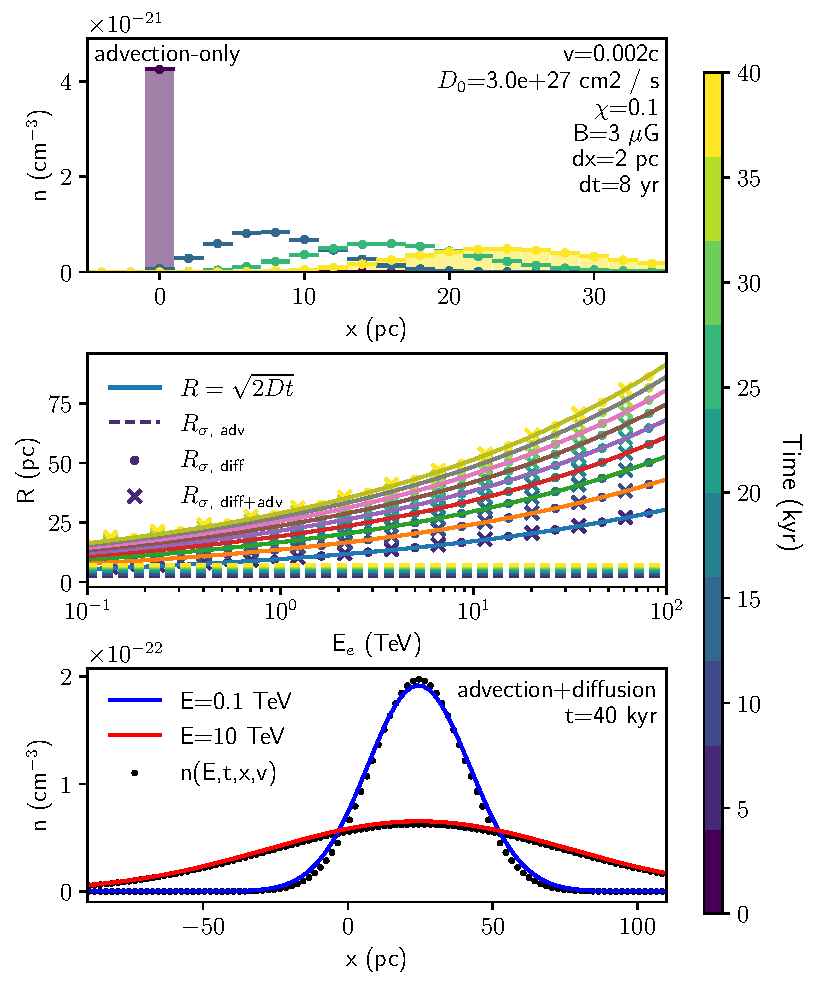
\includegraphics[width=0.7\textwidth]{09_Multizone/Images/advection/advection_1D_multizone_final.pdf}
    \caption{Advection and diffusion of the electron number density with velocity $v=0.002c$ with identical parameters as per \autoref{fig:09_multizone_diff_3D}. (\textit{top}) Dispersion of electrons for an advection-only scenario. (\textit{middle}) A comparison of the 1D diffusive variance radius ($R=\sqrt{2Dt}$) and the radius containing $68\%$ of electrons after advection ($R_{\sigma}$) for an advection-only, diffusion only and diffusion + advection scenarios at different ages of the system. (\textit{bottom}) The numerical (solid lines) and analytical (dots) electron number density distribution at $t=40\,\kiloyear$ for electron energies $E=0.1$ and $10\,\TeV$.}
    \label{fig:09_multizone_adv_multizone_examp}
\end{SCfigure}
Any application of advection to \mbox{HESS\,J1825-137} in this thesis will consider the same parameters as used in \autoref{fig:09_multizone_diff_3D} ($\Delta x =2\,\pc$, $\Delta t=8\,\si{yr}$, $\chi=0.1$, $D_0=3\times 10^{27}\,\si{\centi\meter\squared\per\second}$ and $B=3\,\si{\micro G}$) with an additional an advective velocity of $0.002c$ (see \autoref{sec:10_second_paper}). Therefore, dispersion is negligible compared to diffusion for electrons with energy $\gg 10^{-3}\,\TeV$. The resultant photon from a $10^{-3}\,\TeV$ electron interacting with the CMB via inverse Compton interactions will have energy $\approx 10^{-8}\,\TeV$. Consequently, the dispersion due to the application of finite difference techniques to advection is negligible to the electron and gamma-ray energy range considered in this thesis.

\begin{figure}[h!]
    \centering
    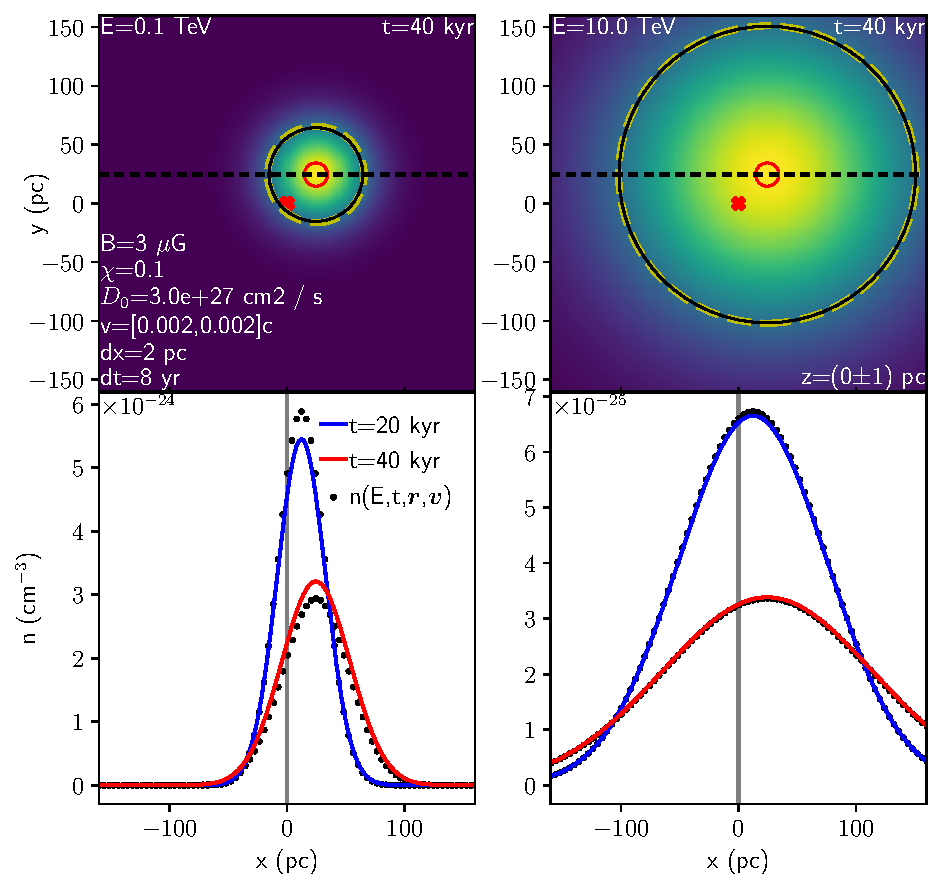
\includegraphics[width=\textwidth]{09_Multizone/Images/advection/advection_2D_multizone_final.pdf}
    \caption{Electron injection into a 2D grid at $x=y=t=0$ and experiencing diffusion and advection with $v=\qty[0.002c,0.002c]$. (\textit{Top}) The number density distribution after $40\,\kiloyear$. The black and yellow dashed circles represent the 2D variance radius ($R_\text{var}$) and the radius containing $1\sigma=68\%$ of electrons ($R_\sigma$) respectively. The red circle describes the $R_\sigma$ containment radius for an advection-only scenario. Finally, the red cross represents the electron source position at $x=y=0$ (\textit{Bottom}) Comparing the numerical solution (lines) and analytical solution (dots, see \autoref{eq:09_multizone_adv_2D_analytical}) at $t=20$ and $40\,\kiloyear$ along $y=(vt\pm 1)\,\pc$ (dashed horizontal line in the bottom panel). The vertical grey line shows the electron source position at $x=0$.}
    \label{fig:09_multizone_adv_2D}
\end{figure}
\newpar 
This dispersion effect can be seen in the top panel of \autoref{fig:09_multizone_adv_multizone_examp}, where electrons are injected at $x=0$ and are transported only though advection at speed $v=0.002c$. After $40\,\kiloyear$, electrons have dispersed with the mean position centred on the voxel corresponding to $d=vt$ with a dispersive radius $R_\sigma\approx 5\,\pc$ containing $68\%$ of electrons. The middle panel of \autoref{fig:09_multizone_adv_multizone_examp} compares the 1D diffusive variance radius ($R=\sqrt{2Dt}$) with $R_\sigma$ for an advection-only scenario, diffusion-only scenario and a diffusion + advection scenario. For electrons within the energy range of interest, $R_{\sigma\text{, adv}}$ is negligible compared to $R_{\sigma\text{, diff}}$. Thus $R_{\sigma\text{, diff+adv}}$ follows the 1D diffusive variance radius. Finally, the bottom panel of \autoref{fig:09_multizone_adv_multizone_examp} compares the numerical solution of diffusion + advection scenario with the analytical solution:

\begin{equation}
    \begin{aligned}
        n_\text{diff+adv}\qty(E,t,x,v)&=n_\text{diff}\qty(E,t,x-vt)\text{ ,} 
    \end{aligned} \label{eq:09_multizone_adv_1D_analytical}
\end{equation}
\noindent for energies $E=0.1$ and $10\,\TeV$ and age $t=40\,\kiloyear$. 
\newpar 
Finite difference methods will now be applied to 2D advection with parameters similar to \autoref{fig:09_multizone_diff_3D} ($\Delta x =2\,\pc$, $\Delta t=8\,\si{yr}$, $\chi=0.1$, $D_0=3\times 10^{27}\,\si{\centi\meter\squared\per\second}$ and $B=3\,\si{\micro G}$) and an advective component $v=\qty[0.002c,0.002c]$ as applied to \mbox{HESS\,J1825-137}. Following \autoref{eq:09_multizone_adv_1D_analytical}, the analytical solution for diffusion + advection is:

\begin{equation}
    \begin{aligned}
        n_\text{diff+adv}\qty(E,t,\vec{r},\vec{v})&=n_\text{diff}\qty(E,t,\vec{r}-\vec{v}t)\text{ ,} 
    \end{aligned} \label{eq:09_multizone_adv_2D_analytical}
\end{equation}
\noindent where $\vec{r}=\qty[x,y,z=50]$, The numerical solution is able to match adequatly the analytical solution as shown in the top panels of \autoref{fig:09_multizone_adv_2D}.


\section{Summary and Application}

In summary, {\tt Multizone} uses finite difference techniques to numerically solve the transport equation in order to predict the electron energy distribution around an accelerator. Isotropic diffusion and spatially independent advection were considered as the main methods of transport. The conditions under which \multizone can match the analytical solution were shown and noted that the dispersive effects due to numerical techniques were negligible for the parameters considered here.
\newpar
Finite difference methods can be used to predict the electron number density in 3D due to advection, where the third dimension is the distance along the line of sight. As discussed in \autoref{appendix:snrs}, the reverse shock of the associated SNR is influenced by the surrounding ISM, where the time the reverse shock takes to form depends on the amount of ISM gas \citep{alma9928040781501811}. The reverse shock, in turn, influences the morphology of the PWN and the preferential direction of electron flow. Figure 2. in \autoref{sec:08} shows the presence of dense gas clouds to the north of \mbox{PSR\,1826-1334} in velocity range $40-60\,\kmpersec$ ($3.5-4.5\,\kpc$). Therefore, the reverse shock will first form to the Galactic north of \mbox{\HESS\,J1825-137} and travel southwards to influence the PWN. Electrons will then be preferentially transported to the Galactic south, resulting the asymmetric gamma-ray morphology seen towards \mbox{HESS\,J1825-137}. Therefore for simplicity, any modelling of \mbox{HESS\,J1825-137} in this thesis will assume a bulk flow of electrons to the Galactic south and zero bulk flow in the line of sight.
\newpar
{\tt Multizone} will be combined with Nanten data (see \autoref{sec:NANTEN}) and magnetic field models to predict the electron energy distribution around \mbox{HESS\,J1825-137} due to pulsar \mbox{PSR\,1826-1334} and the subsequent multi-wavelength morphology. The contamination of nearby $\TeV$ gamma-ray source \mbox{HESS\,J1826-130} (see \autoref{sec:01_1825_1826}) due to \mbox{HESS\,J1825-137} will be investigated. This is summarised in \autoref{sec:10_second_paper}.